\chapter{Complément}
\section{Comparaison simple avec la machine physique}
\begin{figure}[h]
   \begin{minipage}[c]{.46\linewidth}
	   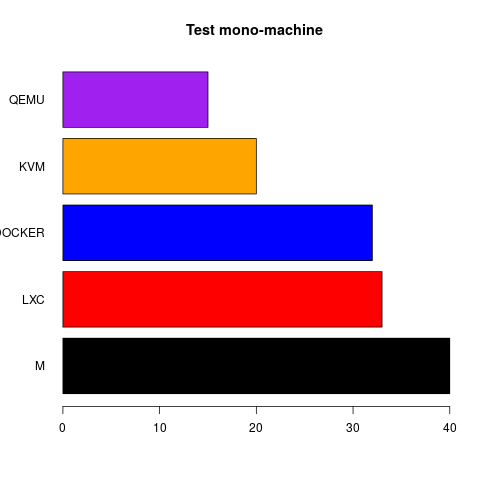
\includegraphics[scale=0.55]{resultats/Monomachine.png}
   \end{minipage} \hfill
   \begin{minipage}[c]{.46\linewidth}
   	Ce graphique est base sur un compte sur l'ensemble des tests avec une seule machine active . La meilleur performance realise par une technologie a un score augmente de 4 puis la deuxième technologie a elle 3, etc.. On constate comme conjecturer plus haut que les conteneurs sont au plus proche des performance réalise par la machine physique (Ici représente par M )
   	 \end{minipage}
\end{figure}
\section{La meilleure technologie?}
\subparagraph{En moyenne ?}
En moyenne, on observe par ordre, que plus le nombre de machines augmente plus KVM se détache suivi d'assez pres par Docker. Ceux-ci sont suivi par LXC puis QEMU .
\subparagraph{Sur chaque scenario}
Sur le scenario du processeur, donc avec les quatre tests mis en œuvre pour évaluer les solutions de virtualisation. LXC, semble être le plus intéressant pour une utilisation CPU.
Sur le scenario de la RAM, Docker et KVM semblent tout deux assez proche avec un nombre de machines active en augmentation.\\
Sur le Web, Docker semble se démarque assez nettement.\\
Sur le HDD, il est assez difficile de distinguer KVM et QEMU qui semble réellement plus constant par rapport au conteneurs.\\
Sur le test de la loopback, il n'y a rien a conclure ce test relise fut totalement inutile et sans intérêt, le seul qui pourrait encore subsister. C'est celui de vérifier que la performance est bien exactement identique sur les différentes solutions de virtualisation.\\
\section{Tentative}
\subsection{Sur les mathématiques}
Plusieurs algorithme de classification et de régression on été tente et réalise pour effectuer plusieurs conjecture grâce a ces outils mathématiques. Ce non résultat est surtout du, au manque de donnée. Il aurais été judicieux de réalise des tests a pas de 1 . La classification et la régression aurait été bien plus intéressante.
\subsection{Sur les tests}
Il a été aussi assez dommage de ne pas pouvoir réalise des test plus avance sur le réseaux, effectivement malgré la présence de test dans la suite Phoronix destine au réseaux. Ceux-ci sont bien connu : 
\begin{itemize}
\item pts/iperf3
\item pts/netperf
\end{itemize}
Malgré l'installation réussite d'un serveur netperf et celui d'un serveur iperf3 .
Il était impossible pour les machines virtuelles de communiquer avec elle lorsque l'orchestration est fait par l'outil phoromatic.
Par contre assez étonnamment avec les mêmes renseignement sur l'adresse et le port d’accès a l’outil phoronix, le lancement manuel fonctionne lui parfaitement.
Il était donc impossible de réalise une orchestration instantanée sur ce benchmark.

De plus il y un test qui malgré plusieurs version n'as jamais ete en capacité d’être lance avec le meme cas de figure pour iperf et netperf. Il s'agit du test hpcc le HPC challenge.
\subsection{Sur les hyperviseurs}
Les hyperviseur/conteneurs on été assez limite, il s'est avéré que il n'y avait pas a disposition une licence Hyper-V.Malgre que un mail fut envoyer pour avoir une license chez Microsoft pour savoir si il était possible de faire un geste, a ce jour ce fut une demande sans réponse. De plus VMWARE n'autorise aucunement la diffusion de résultat comparatif de test . Par conséquent même si il avait été étudie il ne serait a aucun moment donne/ mentionner dans ce rapport de quelconque résultat.